\documentclass[letter, 12pt]{article}

\usepackage{amsmath}
\usepackage{fancyhdr}
\usepackage{geometry}
\usepackage{enumerate}
\usepackage{enumitem}
\usepackage{listings}
\usepackage{algorithm}
\usepackage{algorithmic}
\usepackage{eqparbox}
\usepackage{float}
\usepackage{bm}
\usepackage{bbm}
\usepackage{nccmath, mathtools}
\usepackage{amsthm,amssymb}

\author{Shengjie Li}
\title{Midterm Exam}

\pagestyle{fancy}
\fancyhf{} 
\lhead{Shengjie Li \\ RUID: 188008047}
\cfoot{\thepage} 
\renewcommand{\headrulewidth}{1pt}
\renewcommand{\headwidth}{\textwidth}
\renewcommand\algorithmiccomment[1]{%
	\hfill\#\ \eqparbox{COMMENT}{#1}%
}
\newlist{subquestion}{enumerate}{1}
\setlist[subquestion, 1]{label = \alph*)}
\DeclareMathOperator*{\argmax}{arg\,max}
\DeclareMathOperator*{\argmin}{arg\,min}

\setlength\parindent{0pt}

% margin adjustment
\addtolength{\textwidth}{1in}
\addtolength{\oddsidemargin}{-0.5in}
\addtolength{\evensidemargin}{-0.5in}
\addtolength{\topmargin}{-.5in}
\addtolength{\textheight}{1.0in}
\setlength\parindent{0cm}

\begin{document}
	\centerline{Midterm Exam}
	\begin{enumerate}[wide = 0pt, label = \textbf{Problem \arabic*:}]
		\item {Let $ x_0 $ be deterministic and $ x_1 , \dots , x_N $ denote random variables satisfying (an autoregressive model of order 1)
		\begin{align*}
			x_n = \alpha x_{n-1} + w_n , \ \ n = 1, \dots , N, 
		\end{align*}
		where $ w_1 , \dots , w_N $ are independent and identically distributed Gaussian random variables with mean 0 and variance 1 while $ \alpha $ denotes an unknown parameter. }
		\begin{subquestion}
			\item {Find the joint density of $ x_1 , \dots , x_N $ given $ \alpha $ (remember $ x_0 $ is deterministic).}
			\begin{align*}
				\shortintertext{The joint density function of $ x_1 , \dots , x_N $ is:}
				&f_{X_1 , \dots , X_N}(x_1, x_2, \dots, x_N) \\
				&= f_{X_N | X_1 , \dots , X_{N-1}}(x_N | x_1 , \dots , x_{N-1}) \\
				& \times f_{X_{N-1} | X_1 , \dots , X_{N-2}}(x_{N-1} | x_1 , \dots , x_{N-2}) \\
				& \dots \\
				&\times f_{X_1}(x_1). 
			\end{align*} 
			\begin{align*}
				\shortintertext{Then we can get the CDFs and PDFs:}
				& F_{X_1}(X_1) = P(x_1 < X_1) = P(\alpha x_0 + \omega_1 < X_1) = P(\omega_1 < X_1 - \alpha x_0) = F_w(X_1 - \alpha x_0) \\
				& f_{X_1}(X_1) = f_w(X_1 - \alpha x_0) \\
				& \vdots \\
				& F_{X_N}(X_N) = P(x_N < X_N) = P(\alpha x_{N-1} + \omega_N < X_N) = P(\omega_N < X_N - \alpha x_{N-1}) = F_w(X_N - \alpha x_{N-1}) \\
				& f_{X_N}(X_N) = f_w(X_N - \alpha x_{N-1}) 
			\end{align*}
			\begin{align*}
			\shortintertext{Then the joint density function of $ x_1 , \dots , x_N $ will be:}
				f_{X_1 , \dots , X_N}(x_1, x_2, \dots, x_N) = \prod_{i = 1}^{N}\frac{1}{\sqrt{2\pi}}e^{-\frac{1}{2}(x_i - \alpha x_{i-1})^2} 
			\end{align*} 
		
			\item {Compute the maximum likelihood estimate of $ \alpha $ when you are given $ x_0 $ and a realization of $ x_1 , \dots , x_N. $}
			\begin{align*}
				\shortintertext{From a) we know that}
				\mathcal{L}(\alpha) &= \prod_{i = 1}^{N}\frac{1}{\sqrt{2\pi}}e^{-\frac{1}{2}(x_i - \alpha x_{i-1})^2}.
				\shortintertext{Let $ l(\alpha) = \ln(\mathcal{L}(\alpha)) $,}
				l(\alpha) &= -\frac{N}{2}\ln(2\pi) - \sum_{i = 1}^{N} \frac{1}{2}(x_i - \alpha x_{i-1})^2 \\
				l'(\alpha) &= -\sum_{i = 1}^{N} (x_i - \alpha x_{i-1})(-x_{i-1}) \\
				&= \sum_{i = 1}^{N} (x_i x_{i-1}) - \sum_{i = 1}^{N} (\alpha x_{i-1}^2) \\
				&= \sum_{i = 1}^{N} (x_i x_{i-1}) - \alpha \sum_{i = 1}^{N} (x_{i-1}^2) \\
				l''(\alpha) &= - \sum_{i = 1}^{N} (x_{i-1}^2)
				\shortintertext{Because $ l''(\alpha) = - \sum_{i = 1}^{N} (x_{i-1}^2 < 0$, $ l(\alpha) $ is concave.}
				\shortintertext{Let $ l'(\alpha) = 0$, then we can get the maximum likelihood estimate of $ \alpha $:}
				\alpha &= \frac{\sum_{i = 1}^{N} (x_i x_{i-1})}{ \sum_{i = 1}^{N} (x_{i-1}^2)}. \\
			\end{align*}
		\end{subquestion}
		\item {Let $ x_n , n = 1, \dots , N $ be random variables and consider the two scenarios:  
			\begin{fleqn}[1cm]
				\begin{align*}
				&\mathsf{H}_0 : x_n = -s\alpha_n + w_n, \\
				&\mathsf{H}_1 : x_n = s\alpha_n + w_n,
				\end{align*}
			\end{fleqn}
			 where $ w_n $ are independent and identically distributed Gaussian random variables with mean 0 and variance $ \sigma_2 $ where $ \sigma_2 $ is unknown, $ \alpha_1 , \dots , \alpha_N $ are deterministic and known and, finally $ s > 0 $ is a deterministic and unknown parameter. If the prior probabilities are $ P(\mathsf{H}_0 ) = P(\mathsf{H}_1 ) = 0.5 $ }
		\begin{subquestion}
			\item {Find the optimum decision mechanism that decides between the two scenarios and minimizes the probability of making an error. Start by assuming that all unknown parameters are magically known.}
%			\begin{fleqn}[0cm]
				\begin{gather*}
					 \shortintertext{Let $ D $ be the actual outcome, $ C $ be the cost, then we have:} 
					 \lbrace D_0, H_0 \rbrace \text{ with cost } C_{00}, \\
					 \lbrace D_0, H_1 \rbrace \text{ with cost } C_{01}, \\
					 \lbrace D_1, H_0 \rbrace \text{ with cost } C_{10}, \\
					 \lbrace D_1, H_1 \rbrace \text{ with cost } C_{11}. \\
					 \\
					 \shortintertext{Then the average error(cost) will be:} 
					 C(\delta_0, \delta_1) = C_{00}\mathbb{P}(D_0\&_0) + C_{01}\mathbb{P}(D_0\&_1) + C_{10}\mathbb{P}(D_1\&_0) + C_{11}\mathbb{P}(D_1\&_1). 
				\end{gather*}
				\begin{align*}
					\shortintertext{Let $ C_{00} = C_{11} = 0$, $ C_{01} = C_{10} = 1 $, then} 
					C(\delta_0, \delta_1) &=  \mathbb{P}(D_0 \& H_1) + \mathbb{P}(D_1 \& H_0) \\
					&= \int\delta_0(X)f_1(X)dX \cdot \mathbb{P}(H_1) + \int\delta_1(X)f_0(X)dX \cdot \mathbb{P}(H_0). 
				\end{align*}
				\begin{align*}
					\shortintertext{By definition, we can get:} 
					&F_0(X) = \prod_{i=1}^{N}P(x_i < X_i) = \prod_{i=1}^{N}P(-s\alpha_i + \omega_i < X_i) = \prod_{i=1}^{N}P(\omega_i< X_i +s\alpha_i) = \prod_{i=1}^{N}F_{w_i}(X_i + s\alpha_i) ,\\
					&f_0(X) = \prod_{i=1}^{N}f_{w_i}(X_i + s\alpha_i) .\\
					&F_1(X) = \prod_{i=1}^{N}P(x_i < X_i) = \prod_{i=1}^{N}P(-s\alpha_i - \omega_i < X_i) = \prod_{i=1}^{N}P(\omega_i< X_i -s\alpha_i) = \prod_{i=1}^{N}F_{w_i}(X_i - s\alpha_i) ,\\
					&f_1(X) = \prod_{i=1}^{N}f_{w_i}(X_i - s\alpha_i) .
				\end{align*}
				\begin{align*}
					\shortintertext{We want to minimize the cost, }
					\argmin_{\delta_0, \delta_1} C(\delta_0, \delta_1) &= \argmin_{\delta_0, \delta_1} \int(\delta_0(x)f_1(x)dx \cdot \mathbb{P}(H_1) + \delta_1(x)f_0(x)dx \cdot \mathbb{P}(H_0)). \\
					\\
					\shortintertext{If $ \frac{f_1(x)}{f_0(x)} \ge \frac{\mathbb{P}(H_0)}{\mathbb{P}(H_1)} $, we choose $ H_1 $; If $ \frac{f_1(x)}{f_0(x)} < \frac{\mathbb{P}(H_0)}{\mathbb{P}(H_1)} $, we choose $ H_0 $.}
					\frac{f_1(x)}{f_0(x)} = \frac{\prod_{i=1}^{N}f_w(x_i - s\alpha_i)}{\prod_{i=1}^{N}f_w(x_i + s\alpha_i)} &= \prod_{i=1}^{N} \frac{\frac{1}{\sqrt{2\pi\sigma^2}}e^{-\frac{1}{2\sigma^2}(x_i - s\alpha_i)^2}}{\frac{1}{\sqrt{2\pi\sigma^2}}e^{-\frac{1}{2\sigma^2}(x_i + s\alpha_i)^2}} = \prod_{i=1}^{N} e^{\frac{4x_i s\alpha_i}{2\sigma^2}}
				\end{align*}
%			\end{fleqn}
			The optimum decision mechanism is, if $ \prod_{i=1}^{N} e^{\frac{4x_i s\alpha_i}{2\sigma^2}} \ge 1 $, then we choose $ H_1 $, otherwise we choose $ H_0 $. \\
			
			\item {The decision mechanism you found in a) depends on the unknown parameters $ s $ and $ \sigma_2 $ . Apply suitable transformations to find an equivalent mechanism (by taking for example the logarithm and removing unnecessary terms) which does not depend on these two unknown parameters.} \\
			\\
			From what we got in a), we know that the optimum decision mechanism is, if $ \prod_{i=1}^{N} e^{\frac{4x_i s\alpha_i}{2\sigma^2}} \ge 1 $, then we choose $ H_1 $, otherwise we choose $ H_0 $. \\
			If we do logarithm on both sides, the results would not change.
			\begin{align*}
				& ln(\prod_{i=1}^{N} e^{\frac{4x_i s\alpha_i}{2\sigma^2}}) \ge ln(1) \\
				& \implies \sum_{i=1}^{N} \frac{4x_i s\alpha_i}{2\sigma^2} \ge 0 \\
				& \frac{4s}{2\sigma^2} \sum_{i=1}^{N} x_i \alpha_i \ge 0
				\shortintertext{Because $ s > 0 $, $ \sigma^2 \ge 0 $, }
				& \implies \sum_{i=1}^{N} x_i \alpha_i \ge 0
			\end{align*}
			The equivalent mechanism is: if $ \sum_{i=1}^{N} x_i \alpha_i \ge 0 $, we choose $ H_1 $, otherwise we choose $ H_0 $. \\
			
			\item {Explain what are the optimality properties of the mechanism you ended up with.} 
			\begin{enumerate}
				\item {By using this mechanism, we will have least probability of making an error.}
				\item {Each decision is independent on previous decisions.}
			\end{enumerate}
		\end{subquestion}
	
		\item {Consider a random vector X for which we have three possible scenarios
		\begin{fleqn}[1cm]
			\begin{align*}
			&\mathsf{H}_0 : X \sim f_0 (X),\\
			&\mathsf{H}_1 : X \sim f_1 (X),\\
			&\mathsf{H}_2 : X \sim f_2 (X),
			\end{align*}
		\end{fleqn}
		with all the prior probabilities assumed equal. Find the optimum decision mechanism that minimizes the probability of making an error. Consider now the two likelihood ratios $ \mathsf{L}_1 = \frac{f_1(X)}{f_0(X)} $ and $ \mathsf{L}_2 = \frac{f_2(X)}{f_0(X)} $. For every realization $ X $ you can compute the two likelihood ratios which are in fact all you need to make your
		decision. }
		\begin{subquestion}
			\item {In the 2D space with axes $ \mathsf{L}_1, \mathsf{L}_2 $ identify the regions for which you decide in favor of each of the three scenarios $ \mathsf{H}_0 , \mathsf{H}_1 , \mathsf{H}_2 $ .}
			\begin{align*}
				\shortintertext{Denote the cost of outcome $ i $ and hypothesis $ j $ by $ C_{ij} $.  
				Let 
				$ \begin{cases}
					C_{ij} = 1, i \ne j \\
					C_{ij} = 0, i = j
				\end{cases} $, then we have}
				C(\delta_0, \delta_1, \delta_2) &= \int ((\delta_0 (f_1(x) \mathbb{P}(H_1) + f_2(x) \mathbb{P}(H_2)) + (\delta_1 (f_0(x) \mathbb{P}(H_0) + f_2(x) \mathbb{P}(H_2)) \\
				&+ (\delta_2 (f_0(x) \mathbb{P}(H_0) + f_1(x) \mathbb{P}(H_1))) dx.
				\shortintertext{Because $ {P}(H_0) = {P}(H_1) = {P}(H_2) $, }
				\argmin_{\delta_0, \delta_1, \delta_2} C(\delta_0, \delta_1, \delta_2) &=
				\int ((\delta_0 (f_1(x) + f_2(x)) + (\delta_1 (f_0(x) + f_2(x)) \\
				&+ (\delta_2 (f_0(x) + f_1(x))) dx.
			\end{align*}
			Denote $ f_1(x) + f_2(x) $ by $ C_0 $, $ f_0(x) + f_2(x) $ by $ C_1 $, $ f_0(x) + f_1(x) $ by $ C_2 $, then we can get the optimum decision mechanism: let $ C_i = min(C_0, C_1, C_2) $, set $ \delta_i $ to 1 and any other $ \delta $ to 0. \\
			The region would look like this:
			\begin{figure}[H]
				\centering
				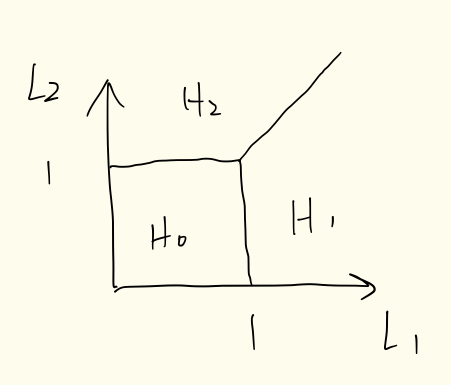
\includegraphics[width=0.5\textwidth]{fig.png}
			\end{figure}
			
			\item {What happens at the boundaries between two regions? What happens at the single point which belongs to the boundary of all three regions?}\\
			\\
			We already knew that all prior probabilities are equal. \\
			Therefore, for $ L_1 = 1 $, we let $ C_i = min(C_0, C_1) $, set $ \delta_i $ to 1 and any other $ \delta $ to 0.\\
			For $ L_2 = 1 $, we let $ C_i = min(C_0, C_2) $, set $ \delta_i $ to 1 and any other $ \delta $ to 0.\\
			For $ L_1 = L_2 $, we let $ C_i = min(C_1, C_2) $, set $ \delta_i $ to 1 and any other $ \delta $ to 0.\\
			For the boundary of all three regions, let $ C_i = min(C_0, C_1, C_2) $, set $ \delta_i $ to 1 and any other $ \delta $ to 0.
		\end{subquestion}
	
		\item {As discussed in the class the space of all random variables constitutes a vector space. We can also define an inner product (also mentioned in class) between two random vectors $ x, y $ 
			\begin{align*}
				<x, y>= E[xy].
			\end{align*} Consider now the following random variables $ x, z, w $. We are interested in linear combinations of the form $ \hat{x}= az + bw $ where a, b are real deterministic quantities.}
		\begin{subquestion}
			\item {By using the orthogonality principle find the $ \hat{x}_\ast $ (equivalently the optimum coefficients $ a_\ast , b _\ast $ ) that is closest to x in the sense of the norm induced by the inner product.}\\
			\\
			Suppose the vector space is $ V = \lbrace y; y = az + bw \rbrace$, $ W $ is a subspace of $ V $. \\
			We want to find the $ \hat{x}_\ast $ that is closest to x, that is:
			\begin{align*}
				&\argmin_{\hat{x}} || x - \hat{x} ||, <x - \hat{x}, y> = 0 \text{ for all $ y $ in $ W $}.
				\shortintertext{Then we can get}
				&<x - \hat{x}, z> = <x - \hat{x}, w> = 0 \\
				&<x - \hat{x}, z> = <x - (az + bw), z> = E[(x - (az + bw))z] = E[xz] - aE[z^2] - bE[wz] = 0 \\
				&E[xz] = aE[z^2] - bE[wz] \\
				&<x - \hat{x}, w> = <x - (az + bw), w> = E[(x - (az + bw))w] = E[xw] - aE[z^2] - bE[wz] = 0 \\
				&E[xw] = aE[zw] - bE[w^2] \\
				&a_{\ast} = \frac{E[xz]E[w^2] - E[xw]E[wz]}{E[z^2]E[w^2] - E[wz]^2} \\
				&b_{\ast} = \frac{E[xw]E[z^2] - E[xz]E[wz]}{E[z^2]E[w^2] - E[wz]^2}
			\end{align*}
			
			\item {Compute the optimum (minimum) distance and its optimum approximation $ \hat{x}_\ast $ in terms of $ E[xz], E[xw], E[z^2 ], E[zw], E[w^2] $.}
			\item {Explain what is the physical meaning of this approximation.}
		\end{subquestion}
	\end{enumerate}
\end{document}
